% style/preamble throws error, hence preamble4tex is kept here
\documentclass[11pt,compress,t,notes=noshow, xcolor=table]{beamer}
\usepackage[]{graphicx}\usepackage[]{color}
% maxwidth is the original width if it is less than linewidth
% otherwise use linewidth (to make sure the graphics do not exceed the margin)
\makeatletter
\def\maxwidth{ %
  \ifdim\Gin@nat@width>\linewidth
    \linewidth
  \else
    \Gin@nat@width
  \fi
}
\makeatother

\definecolor{fgcolor}{rgb}{0.345, 0.345, 0.345}
\newcommand{\hlnum}[1]{\textcolor[rgb]{0.686,0.059,0.569}{#1}}%
\newcommand{\hlstr}[1]{\textcolor[rgb]{0.192,0.494,0.8}{#1}}%
\newcommand{\hlcom}[1]{\textcolor[rgb]{0.678,0.584,0.686}{\textit{#1}}}%
\newcommand{\hlopt}[1]{\textcolor[rgb]{0,0,0}{#1}}%
\newcommand{\hlstd}[1]{\textcolor[rgb]{0.345,0.345,0.345}{#1}}%
\newcommand{\hlkwa}[1]{\textcolor[rgb]{0.161,0.373,0.58}{\textbf{#1}}}%
\newcommand{\hlkwb}[1]{\textcolor[rgb]{0.69,0.353,0.396}{#1}}%
\newcommand{\hlkwc}[1]{\textcolor[rgb]{0.333,0.667,0.333}{#1}}%
\newcommand{\hlkwd}[1]{\textcolor[rgb]{0.737,0.353,0.396}{\textbf{#1}}}%
\let\hlipl\hlkwb

\usepackage{framed}
\makeatletter
\newenvironment{kframe}{%
 \def\at@end@of@kframe{}%
 \ifinner\ifhmode%
  \def\at@end@of@kframe{\end{minipage}}%
  \begin{minipage}{\columnwidth}%
 \fi\fi%
 \def\FrameCommand##1{\hskip\@totalleftmargin \hskip-\fboxsep
 \colorbox{shadecolor}{##1}\hskip-\fboxsep
     % There is no \\@totalrightmargin, so:
     \hskip-\linewidth \hskip-\@totalleftmargin \hskip\columnwidth}%
 \MakeFramed {\advance\hsize-\width
   \@totalleftmargin\z@ \linewidth\hsize
   \@setminipage}}%
 {\par\unskip\endMakeFramed%
 \at@end@of@kframe}
\makeatother

\definecolor{shadecolor}{rgb}{.97, .97, .97}
\definecolor{messagecolor}{rgb}{0, 0, 0}
\definecolor{warningcolor}{rgb}{1, 0, 1}
\definecolor{errorcolor}{rgb}{1, 0, 0}
\newenvironment{knitrout}{}{} % an empty environment to be redefined in TeX

\usepackage{alltt}
\newcommand{\SweaveOpts}[1]{}  % do not interfere with LaTeX
\newcommand{\SweaveInput}[1]{} % because they are not real TeX commands
\newcommand{\Sexpr}[1]{}       % will only be parsed by R
\newcommand{\xmark}{\ding{55}}%


\usepackage[english]{babel}
\usepackage[utf8]{inputenc}

\usepackage{dsfont}
\usepackage{verbatim}
\usepackage{amsmath}
\usepackage{amsfonts}
\usepackage{amssymb}
\usepackage{bm}
\usepackage{csquotes}
\usepackage{multirow}
\usepackage{longtable}
\usepackage{booktabs}
\usepackage{enumerate}
\usepackage[absolute,overlay]{textpos}
\usepackage{psfrag}
\usepackage{algorithm}
\usepackage{algpseudocode}
\usepackage{eqnarray}
\usepackage{arydshln}
\usepackage{tabularx}
\usepackage{placeins}
\usepackage{tikz}
\usepackage{setspace}
\usepackage{colortbl}
\usepackage{mathtools}
\usepackage{wrapfig}
\usepackage{bm}
\usepackage{amsmath}
\usepackage{pifont}
\usepackage{xcolor} %colored math symbols

\usetikzlibrary{shapes,arrows,automata,positioning,calc,chains,trees, shadows}
\tikzset{
  %Define standard arrow tip
  >=stealth',
  %Define style for boxes
  punkt/.style={
    rectangle,
    rounded corners,
    draw=black, very thick,
    text width=6.5em,
    minimum height=2em,
    text centered},
  % Define arrow style
  pil/.style={
    ->,
    thick,
    shorten <=2pt,
    shorten >=2pt,}
}

\usepackage{subfig}

% Defines macros and environments
\usepackage{../../style/lmu-lecture}


\let\code=\texttt
\let\proglang=\textsf

\setkeys{Gin}{width=0.9\textwidth}

\setbeamertemplate{frametitle}{\expandafter\uppercase\expandafter\insertframetitle}

\usepackage{bbm}
% basic latex stuff
\newcommand{\pkg}[1]{{\fontseries{b}\selectfont #1}} %fontstyle for R packages
\newcommand{\lz}{\vspace{0.5cm}} %vertical space
\newcommand{\dlz}{\vspace{1cm}} %double vertical space
\newcommand{\oneliner}[1] % Oneliner for important statements
{\begin{block}{}\begin{center}\begin{Large}#1\end{Large}\end{center}\end{block}}


%new environments
\newenvironment{vbframe}  %frame with breaks and verbatim
{
 \begin{frame}[containsverbatim,allowframebreaks]
}
{
\end{frame}
}

\newenvironment{vframe}  %frame with verbatim without breaks (to avoid numbering one slided frames)
{
 \begin{frame}[containsverbatim]
}
{
\end{frame}
}

\newenvironment{blocki}[1]   % itemize block
{
 \begin{block}{#1}\begin{itemize}
}
{
\end{itemize}\end{block}
}

\newenvironment{fragileframe}[2]{  %fragile frame with framebreaks
\begin{frame}[allowframebreaks, fragile, environment = fragileframe]
\frametitle{#1}
#2}
{\end{frame}}


\newcommand{\myframe}[2]{  %short for frame with framebreaks
\begin{frame}[allowframebreaks]
\frametitle{#1}
#2
\end{frame}}

\newcommand{\remark}[1]{
  \textbf{Remark:} #1
}


\newenvironment{deleteframe}
{
\begingroup
\usebackgroundtemplate{
\includegraphics[width=\paperwidth,height=\paperheight]{../style/color/red.png}}
 \begin{frame}
}
{
\end{frame}
\endgroup
}
\newenvironment{simplifyframe}
{
\begingroup
\usebackgroundtemplate{
\includegraphics[width=\paperwidth,height=\paperheight]{../style/color/yellow.png}}
 \begin{frame}
}
{
\end{frame}
\endgroup
}\newenvironment{draftframe}
{
\begingroup
\usebackgroundtemplate{
\includegraphics[width=\paperwidth,height=\paperheight]{../style/color/green.jpg}}
 \begin{frame}
}
{
\end{frame}
\endgroup
}
% https://tex.stackexchange.com/a/261480: textcolor that works in mathmode
\makeatletter
\renewcommand*{\@textcolor}[3]{%
  \protect\leavevmode
  \begingroup
    \color#1{#2}#3%
  \endgroup
}
\makeatother


\input{../../latex-math/basic-math}
\input{../../latex-math/basic-ml}
\input{../../latex-math/ml-nn}

\newcommand{\titlefigure}{figure/front.png} %modify picture
\newcommand{\learninggoals}{
  \item What are CNNs?
  \item When to apply CNNs?
  \item A glimpse into CNN architectures
}

\title{Deep Learning}
\date{}

\begin{document}

\lecturechapter{CNN: Introduction}
\lecture{I2DL}
%%%%%%%%%%%%%%%%%%%%%%%%%%%%%%%%%%%%%%%%%%%%%%%%%%%%%%%%%%%%%%%%%%

\begin{vbframe}{Convolutional Neural Networks}
\begin{itemize}
\item Convolutional Neural Networks (CNN, or ConvNet) are a powerful family of neural networks that are inspired by biological processes in which the connectivity pattern between neurons resembles the organization of the mamel visual cortex.
\end{itemize}
\begin{figure}
\centering
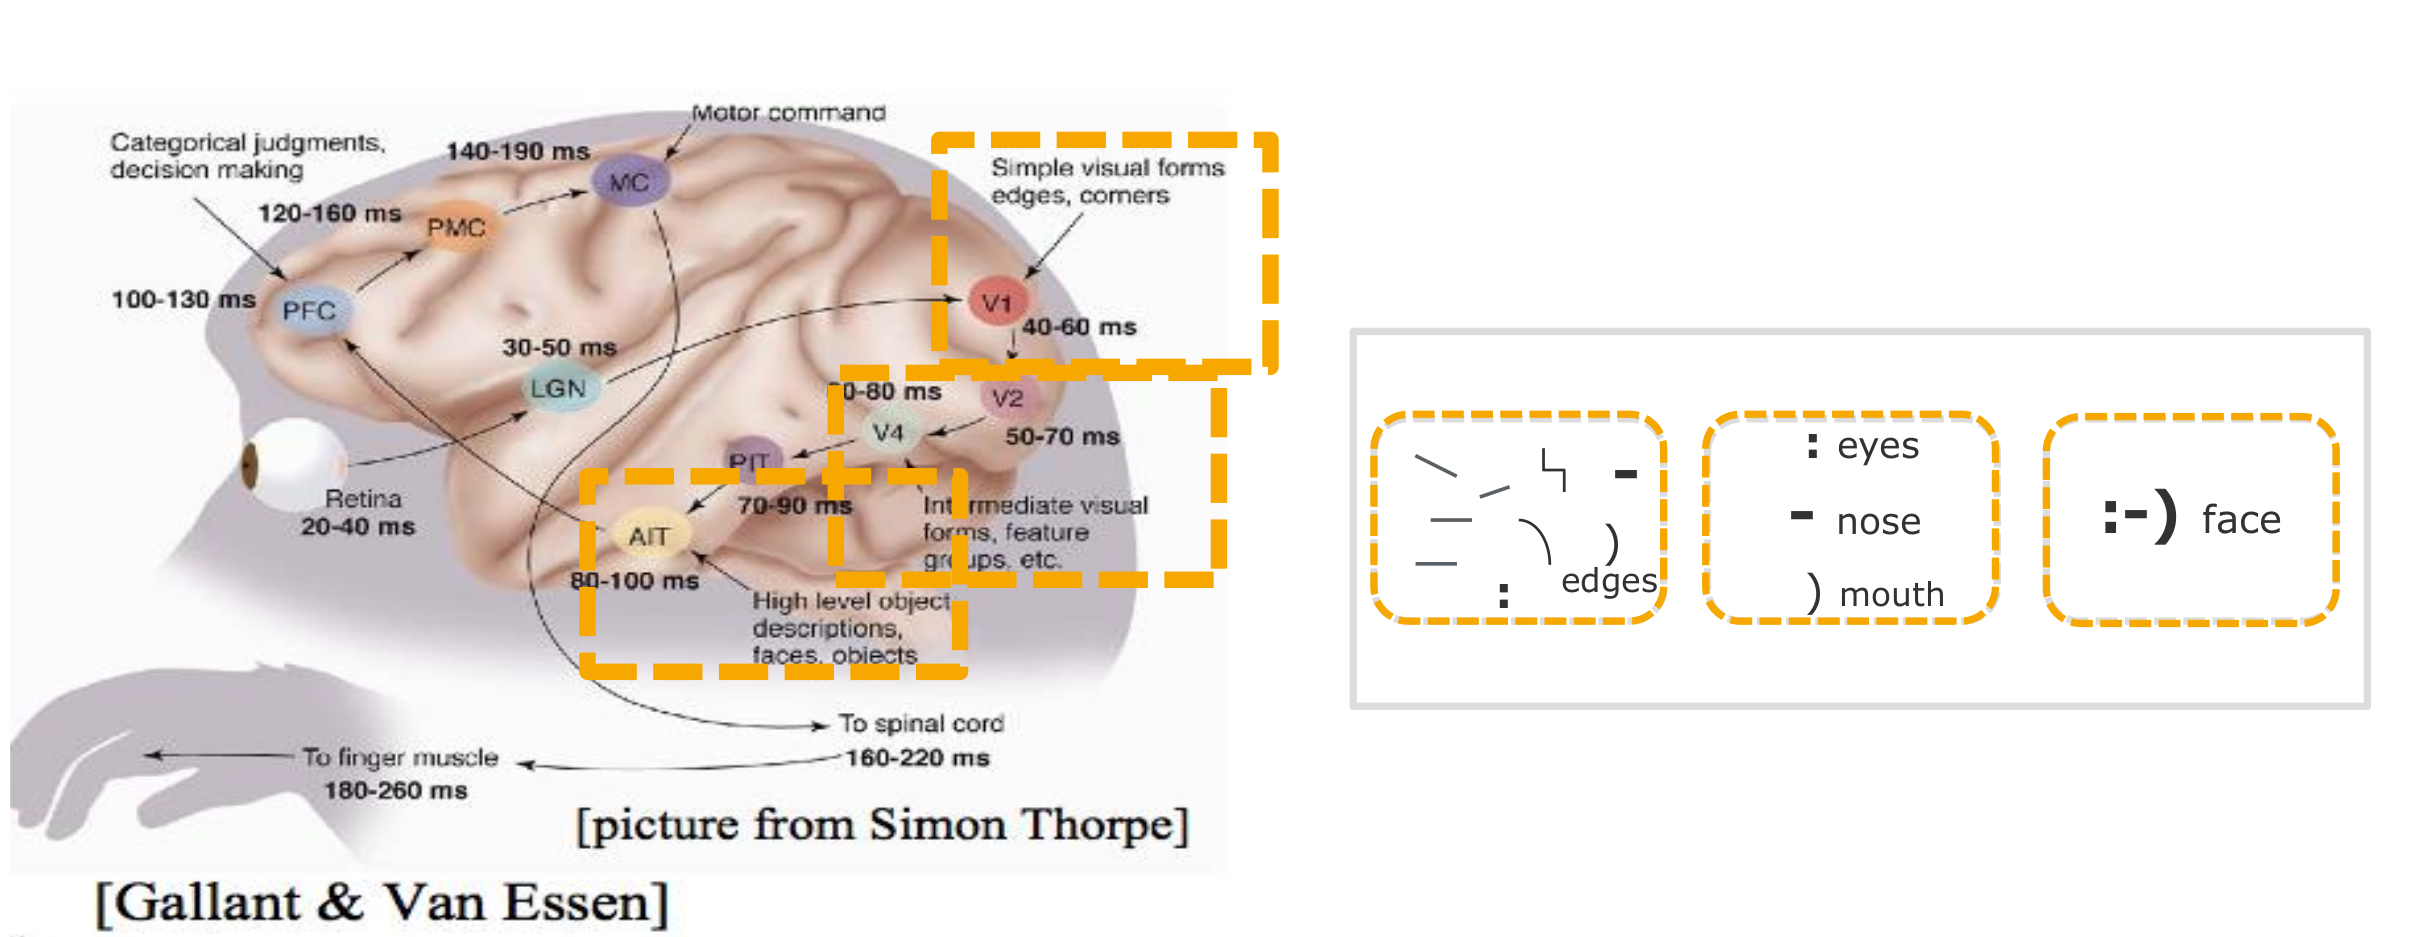
\includegraphics[width=8cm]{figure/cortex.png}
\caption{The ventral (recognition) pathway in the visual cortex has multiple stage: Retina - LGN - V1 - V2 - V4 - PIT - AIT etc., which consist of lots of intermediate representations.}
\end{figure}
\framebreak
%%%%%%%%%%%%%%%%%%%%%%%%%%%%%%%%%%%%%%%%%%%%%%%%%%%%%%%%%%%%%%%%%%

\begin{itemize}
    \item Since 2012, given their success in the ILSVRC competition, CNNs are popular in many fields.
    \item Common applications of CNN-based architectures in computer vision are:
    \begin{itemize}
      \item Image classification.
      \item Object detection / localization.
      \item Semantic segmentation.
    \end{itemize}
    \item CNNs are widely applied in other domains such as natural language processing (NLP), audio, and time-series data.
\item Basic idea: a CNN automatically extracts visual, or, more generally, spatial features from an input data such that it is able to make the optimal prediction based on the extracted features.
\item It contains different building blocks and components. 
\end{itemize}
\end{vbframe}

%%%%%%%%%%%%%%%%%%%%%%%%%%%%%%%%%%%%%%%%%%%%%%%%%%%%%%%%%%%%%%%%%%

\begin{vbframe}{CNNs - What for?}
  \begin{figure}
    \centering
    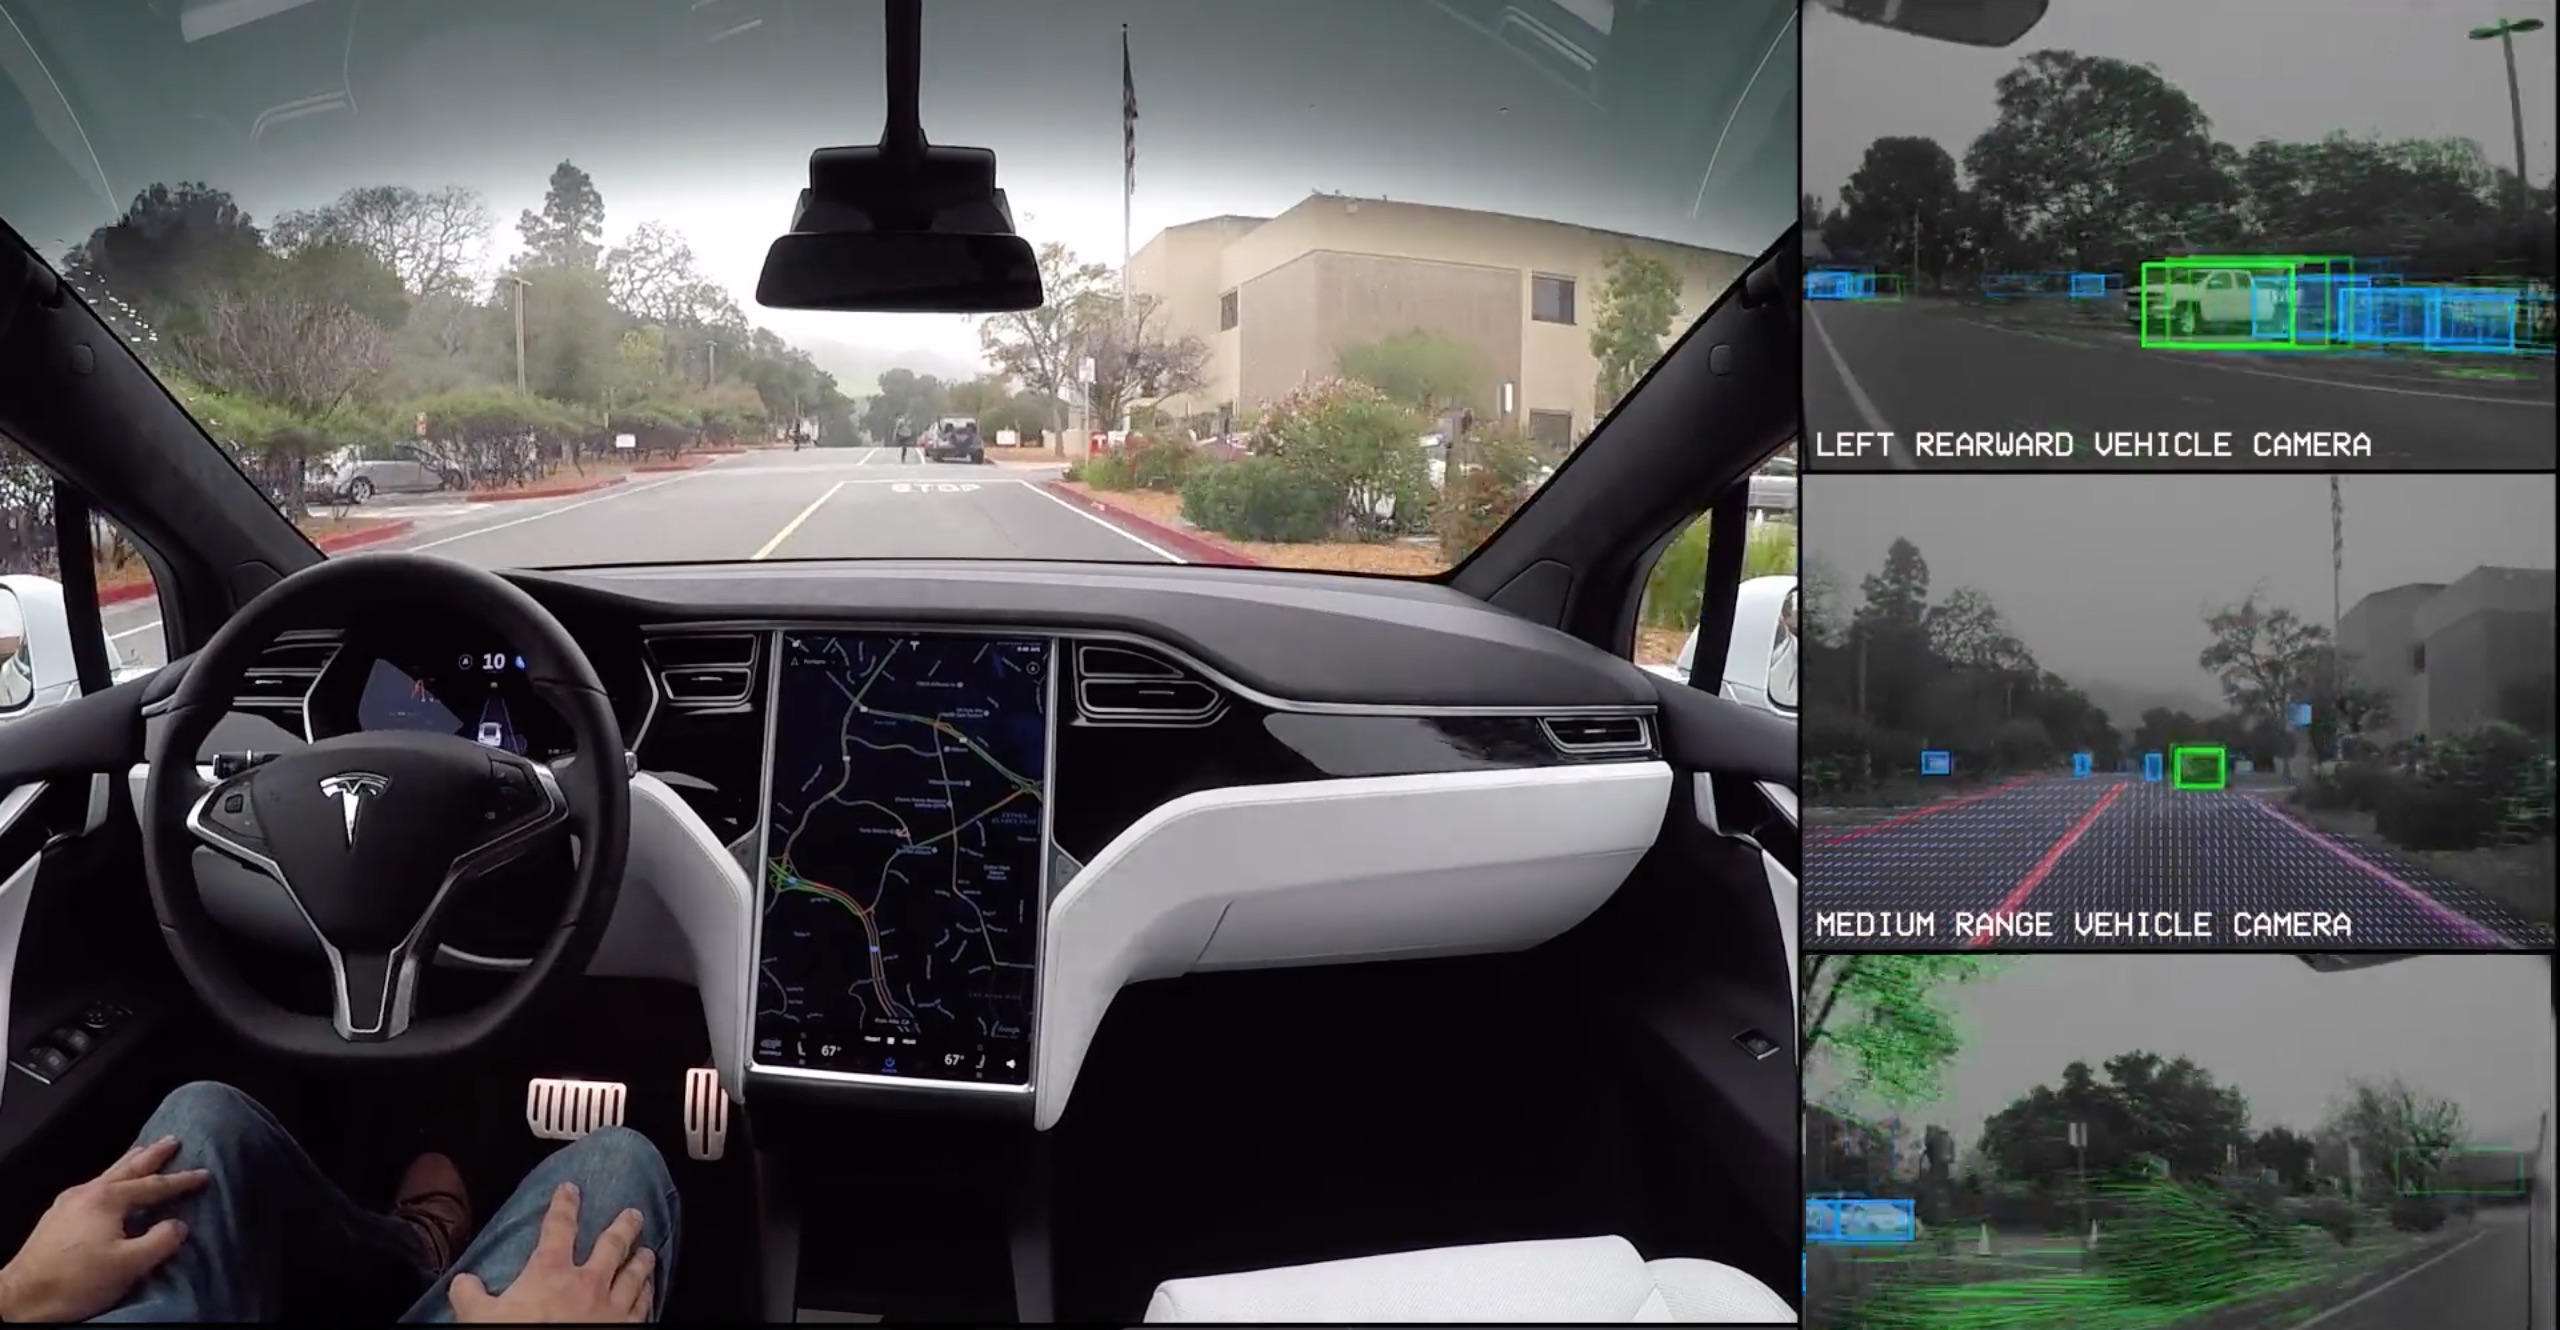
\includegraphics[width=7cm]{figure/tesla_autopilot.jpg}
    \caption{All Tesla cars being produced now have full self-driving hardware (Source: Tesla website). A convolutional neural network is used to map raw pixels from a single front-facing camera directly into steering commands. The system learns to drive in traffic, on local roads, with or without lane markings as well as on highways.}
  \end{figure}
\framebreak
%%%%%%%%%%%%%%%%%%%%%%%%%%%%%%%%%%%%%%%%%%%%%%%%%%%%%%%%%%%%%%%%%%

\begin{figure}
    \centering
    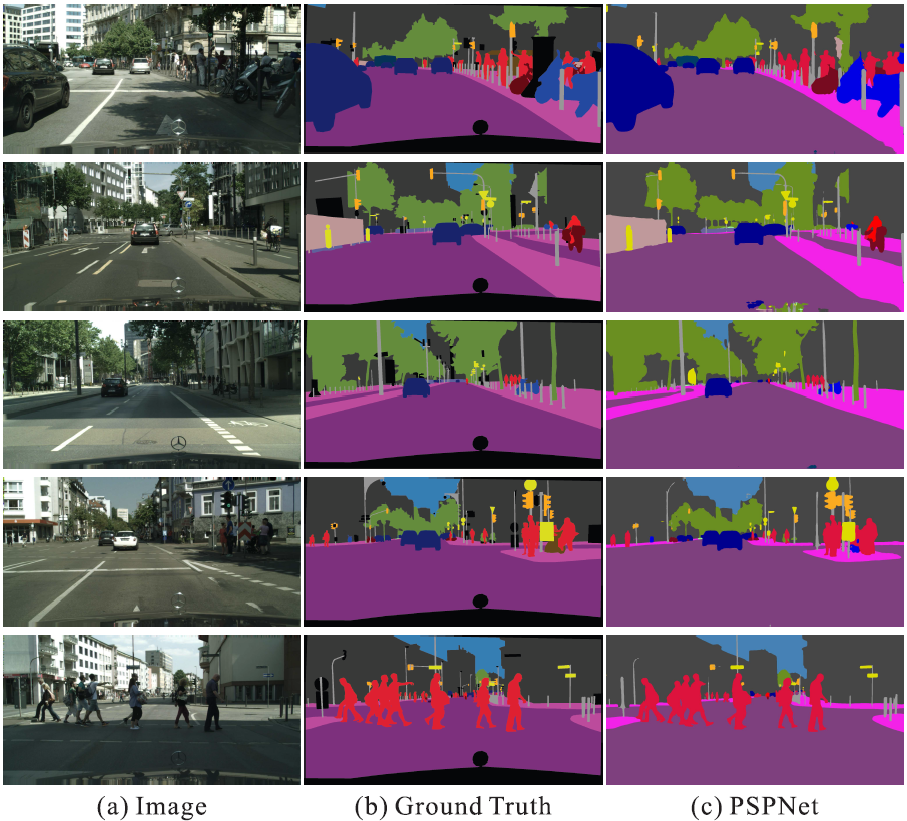
\includegraphics[width=5cm]{figure/cityscapes_visual.png}
    \caption{Given an input image, a CNN is first used to get the feature map of the last convolutional layer, then a pyramid parsing module is applied to harvest different sub-region representations, followed by upsampling and concatenation layers to form the final feature representation, which carries both local and global context information. Finally, the representation is fed into a convolution layer to get the final per-pixel prediction. (Source: pyramid scene parsing network, by Zhao et. al, CVPR 2017) }%mina modify the caption of this figure % DR: way too complicated
  \end{figure}
\framebreak
%%%%%%%%%%%%%%%%%%%%%%%%%%%%%%%%%%%%%%%%%%%%%%%%%%%%%%%%%%%%%%%%%%

  \begin{figure}
    \centering
    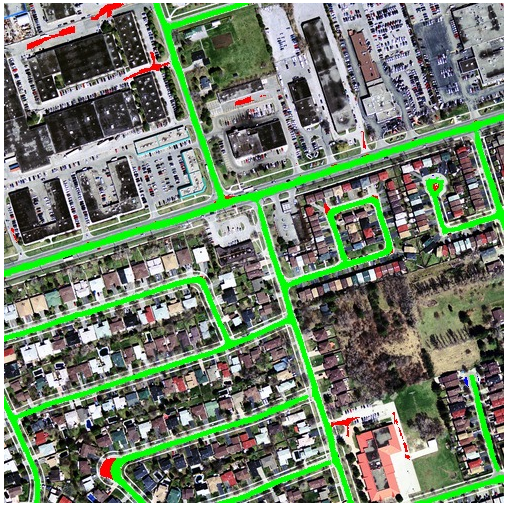
\includegraphics[width=6cm]{figure/road_seg.png}
    \caption{Road segmentation (Mnih Volodymyr (2013)). Aerial images and possibly outdated map pixels are segmented.}
  \end{figure}
\framebreak
%%%%%%%%%%%%%%%%%%%%%%%%%%%%%%%%%%%%%%%%%%%%%%%%%%%%%%%%%%%%%%%%%%

\begin{wrapfigure}{R}{0.5\textwidth}
  \centering
  \scalebox{0.5}{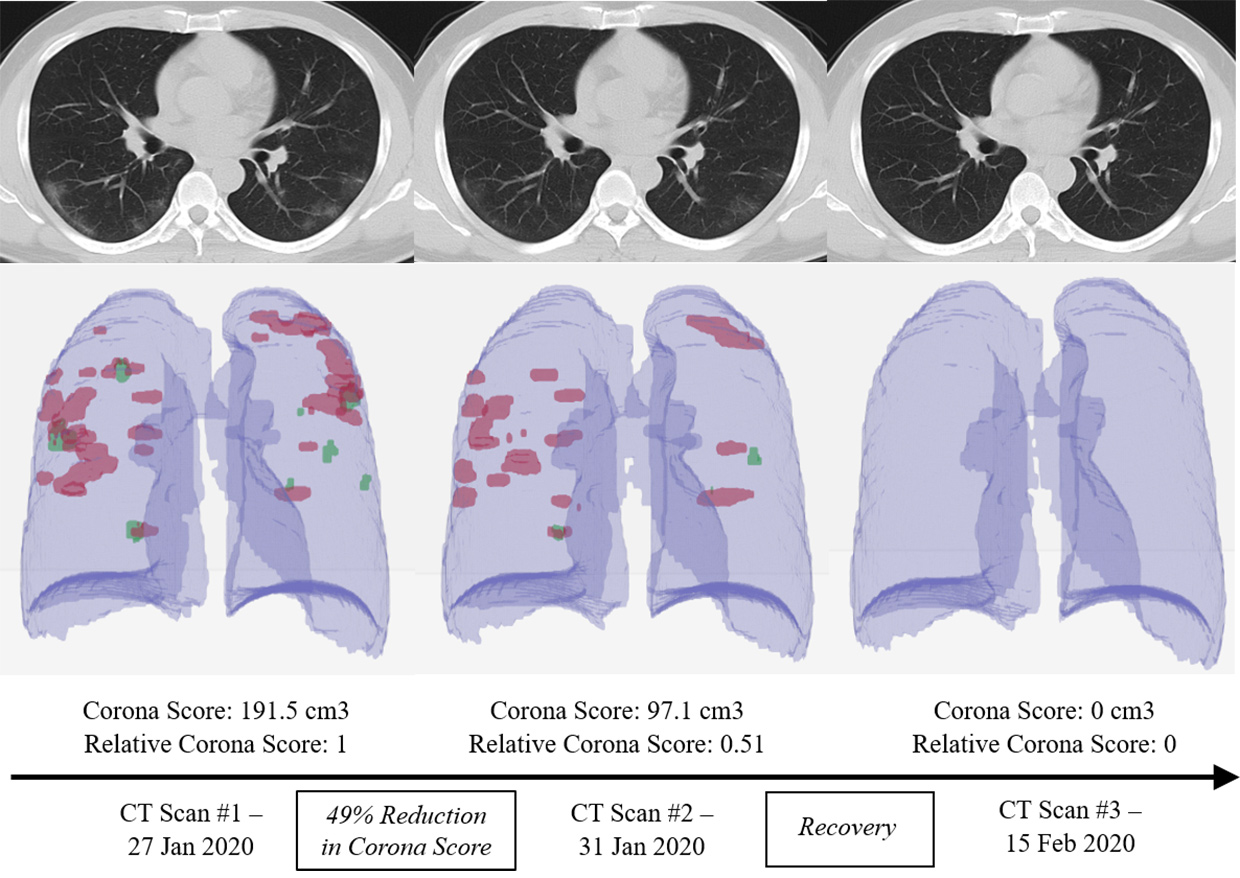
\includegraphics{figure/coronatrack.jpeg}}
\end{wrapfigure}

{CNN for personalized medicine}
  \begin{itemize}
    \item Examples: Tracking, diagnosis and localization of Covid-19 patients.
    \item CNN based method (RADLogists) for personalized Covid-19 detection: three CT scans from a single Corona virus patient diagnosed by RADLogists. % DR: what is RADLogists? Google search gives 0 results
  \end{itemize}
  
   \begin{figure}
    \centering
    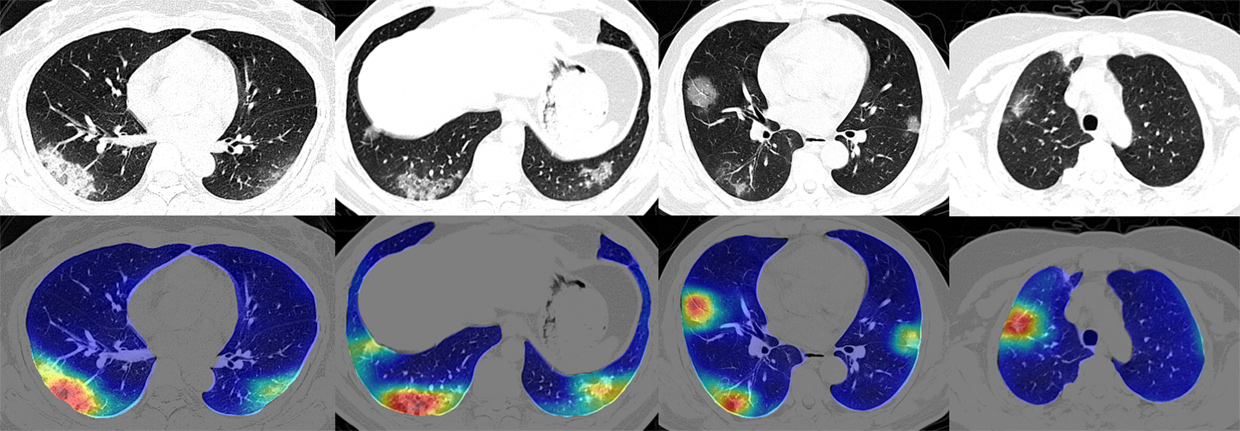
\includegraphics[width=9cm]{figure/hitmap.jpeg}
    \caption{Four COVID-19 lung CT scans at the top with corresponding colored maps showing Corona virus abnormalities at the bottom (Source: Megan Scudellari, IEEE Spectrum 2021).}
  \end{figure}
\framebreak
%%%%%%%%%%%%%%%%%%%%%%%%%%%%%%%%%%%%%%%%%%%%%%%%%%%%%%%%%%%%%%%%%%

  \begin{figure}
    \centering
    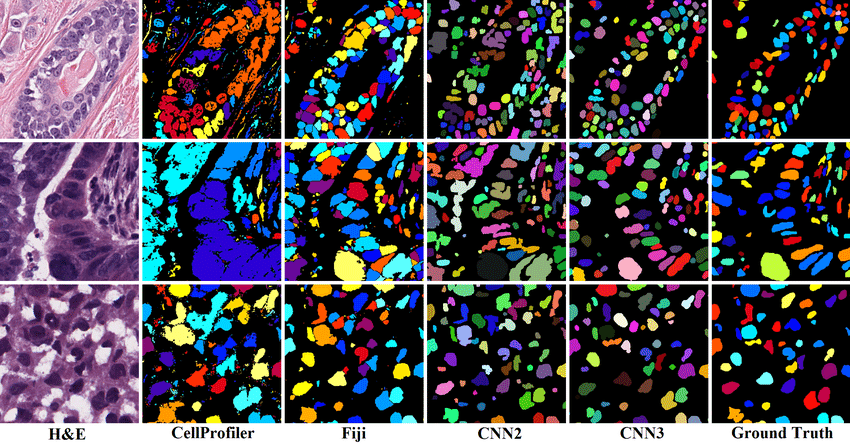
\includegraphics[width=9cm]{figure/instanceseg.png}
    \caption{Various analyses in computational pathology are possible. For example, nuclear segmentation in digital microscopic tissue images enable extraction of high-quality features for nuclear morphometrics (Source: Kummar et. al. IEEE Transaction Medical Imaging). }
  \end{figure}
\framebreak
%%%%%%%%%%%%%%%%%%%%%%%%%%%%%%%%%%%%%%%%%%%%%%%%%%%%%%%%%%%%%%%%%%

  \begin{figure}
    \centering
    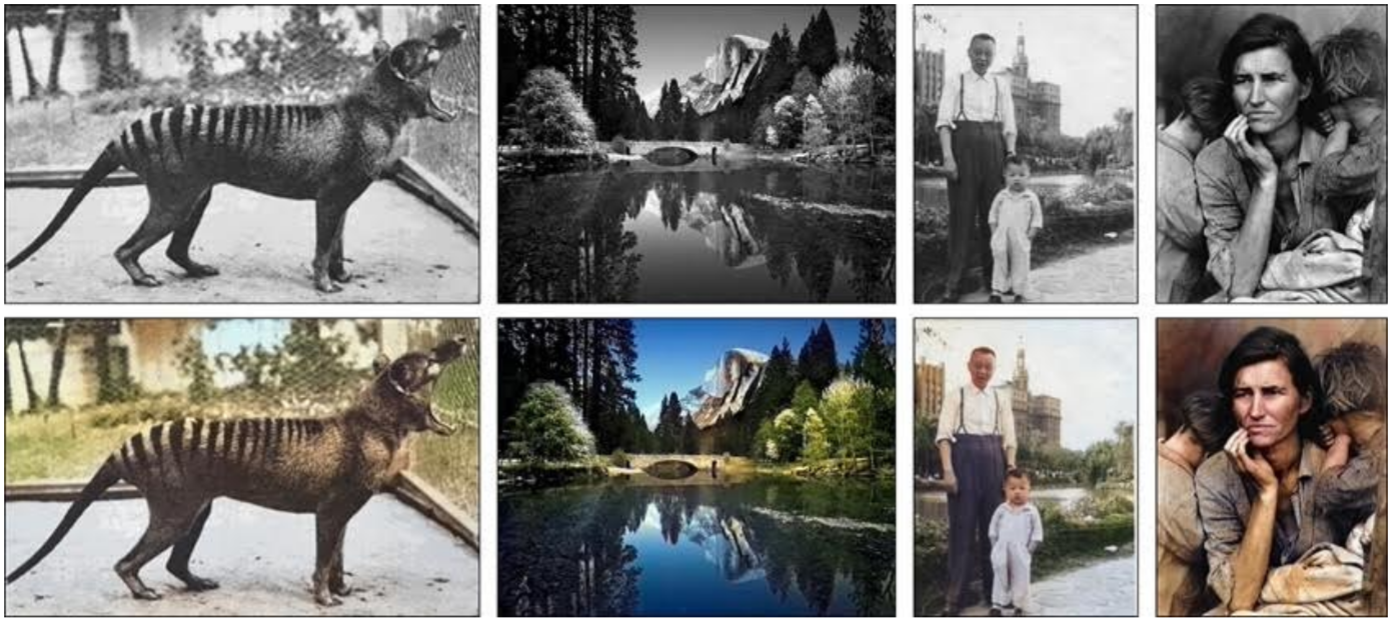
\includegraphics[width=11cm]{figure/colorization.png}
    \caption{Image Colorization is another interesting application of CNN in computer vision (Zhang et al. (2016)). Given a grayscale photo as the input (top row), this network solves the problem of hallucinating a plausible color version of the photo (bottom row, i.e. the prediction of the network).}
  \end{figure}
\framebreak

%%%%%%%%%%%%%%%%%%%%%%%%%%%%%%%%%%%%%%%%%%%%%%%%%%%%%%%%%%%%%%%%%%

  \begin{figure}
    \centering
    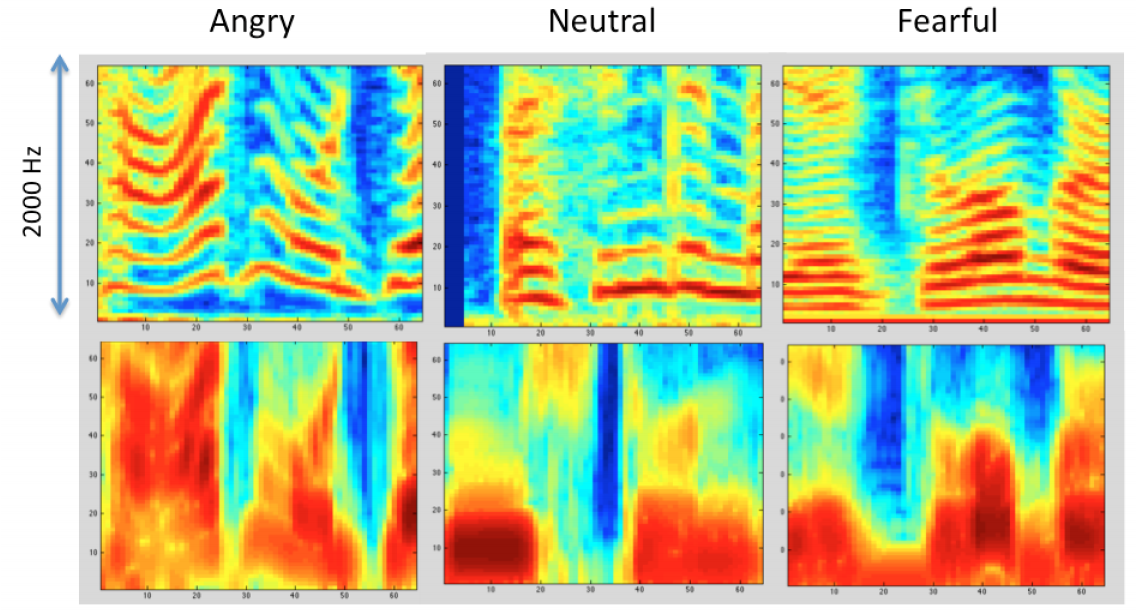
\includegraphics[width=10cm]{figure/speech.png}
    \caption{Speech recognition (Anand \& Verma (2015)). Convolutional neural network is used to learn features from the audio data in order to classify emotions.}
  \end{figure}
\end{vbframe}
%%%%%%%%%%%%%%%%%%%%%%%%%%%%%%%%%%%%%%%%%%%%%%%%%%%%%%%%%%%%%%%%%%

\begin{frame}{CNNs - A First Glimpse} 
\center
\only<1>{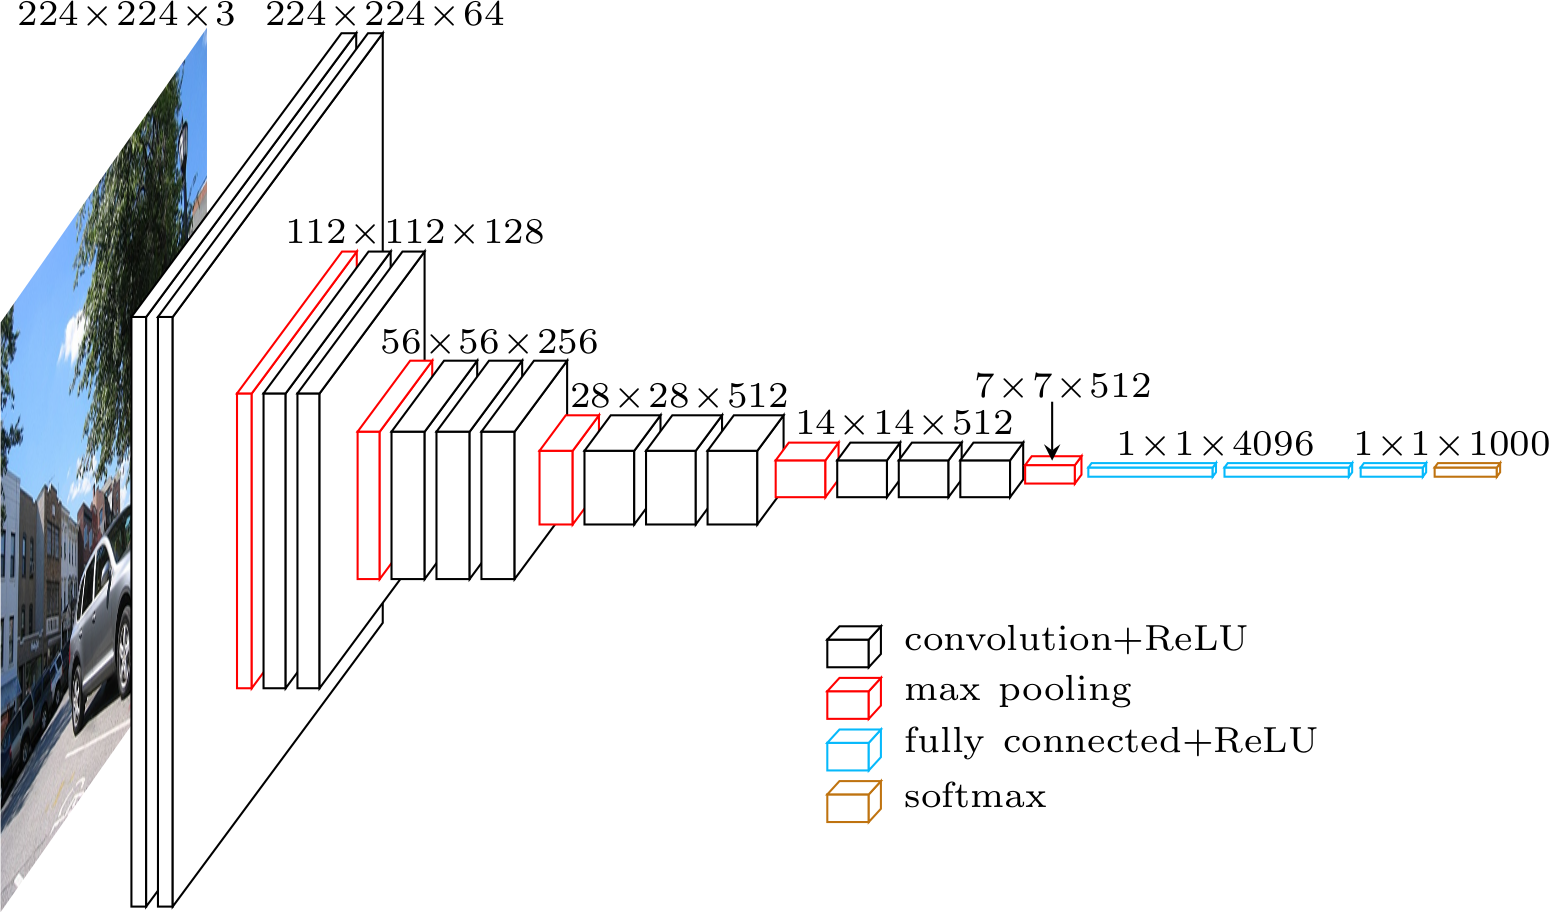
\includegraphics[width=9cm]{figure/alexnet.png}}%
\only<2>{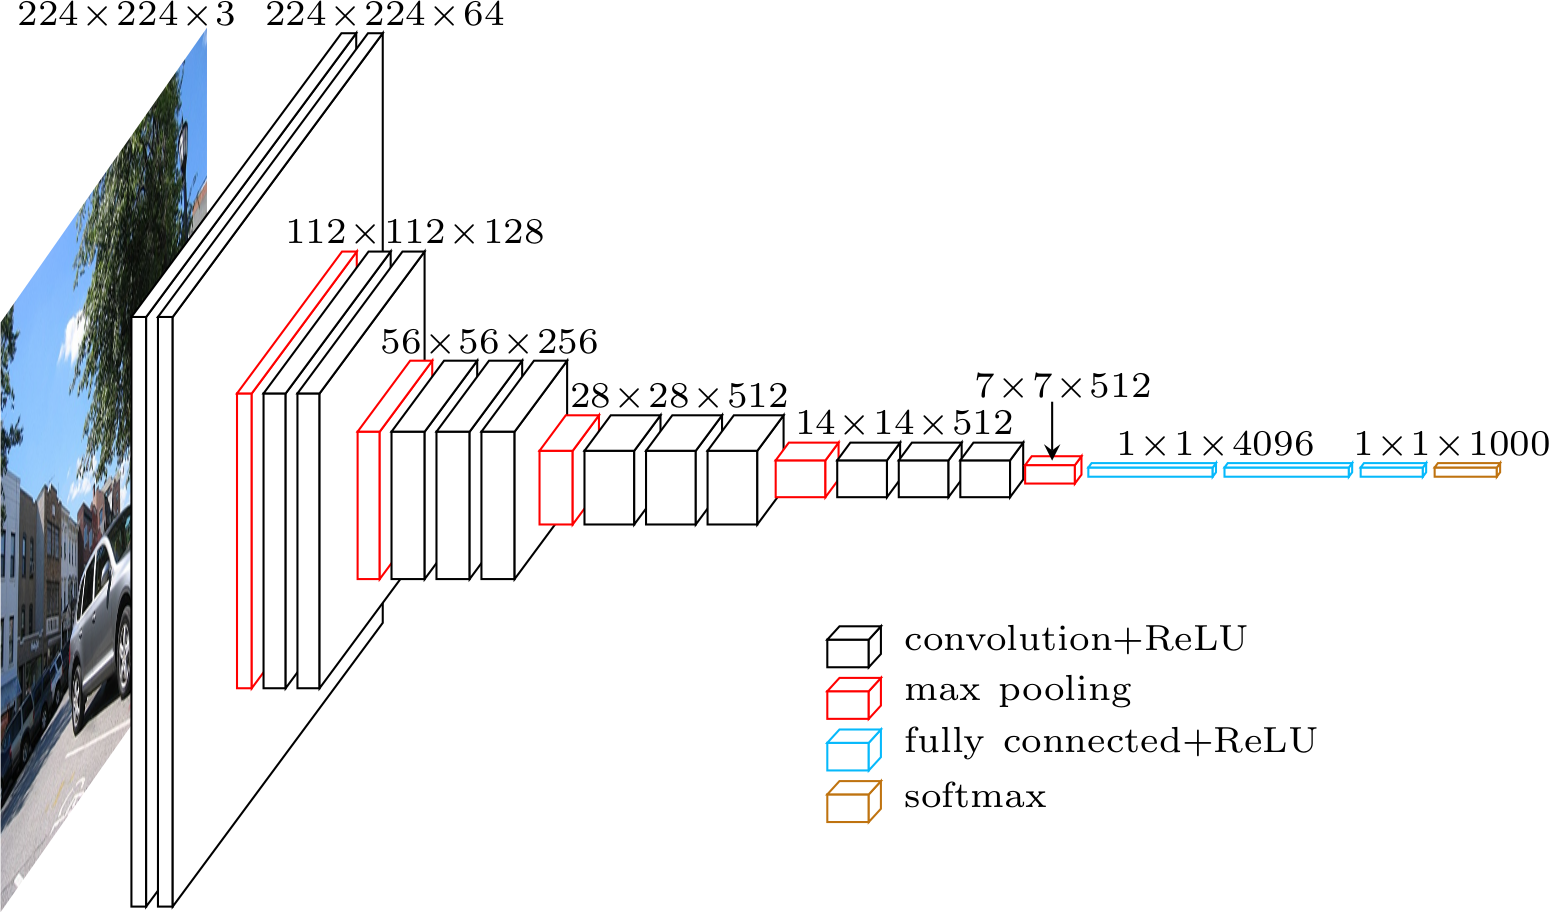
\includegraphics[width=9cm]{figure/alexnet.png}}%
\begin{itemize}
\only<1>{\item \textbf{Input layer} takes input data (e.g. image, audio).}
\only<1>{\item \textbf{Convolution layers} extract feature maps from the previous layers.}
\only<1>{\item \textbf{Pooling layers} reduce the dimensionality of feature maps and filter meaningful features.}
\only<2>{\item \textbf{Fully connected layers} connect feature map elements to the output neurons.}
\only<2>{\item \textbf{Softmax} converts output values to probability scores.}
\end{itemize}
\end{frame}
%%%%%%%%%%%%%%%%%%%%%%%%%%%%%%%%%%%%%%%%%%%%%%%%%%%%%%%%%%%%%%%%%%

\endlecture
\end{document}